%\iffalse
\let\negmedspace\undefined
\let\negthickspace\undefined
\documentclass[journal,12pt,twocolumn]{IEEEtran}
\usepackage{cite}
\usepackage{amsmath,amssymb,amsfonts,amsthm}
\usepackage{algorithmic}
\usepackage{graphicx}
\usepackage{textcomp}
\usepackage{xcolor}
\usepackage{txfonts}
\usepackage{listings}
\usepackage{enumitem}
\usepackage{mathtools}
\usepackage{gensymb}
\usepackage{comment}
\usepackage[breaklinks=true]{hyperref}
\usepackage{tkz-euclide} 
\usepackage{listings}
\usepackage{gvv}                                        
\def\inputGnumericTable{}                                 
\usepackage[latin1]{inputenc}                                
\usepackage{color}                                            
\usepackage{array}                                            
\usepackage{longtable}                                       
\usepackage{calc}                                             
\usepackage{multirow}                                         
\usepackage{hhline}                                           
\usepackage{ifthen}                                           
\usepackage{lscape}

\newtheorem{theorem}{Theorem}[section]
\newtheorem{problem}{Problem}
\newtheorem{proposition}{Proposition}[section]
\newtheorem{lemma}{Lemma}[section]
\newtheorem{corollary}[theorem]{Corollary}
\newtheorem{example}{Example}[section]
\newtheorem{definition}[problem]{Definition}
\newcommand{\BEQA}{\begin{eqnarray}}
 \newcommand{\EEQA}{\end{eqnarray}}
\newcommand{\define}{\stackrel{\triangle}{=}}
\theoremstyle{remark}
\newtheorem{rem}{Remark}
\begin{document}
 \bibliographystyle{IEEEtran}
 \vspace{3cm}
 \title{\textbf{XE 71}}
 \author{EE23BTECH11048-Ponugumati Venkata Chanakya$^{*}$% <-this % stops a space
 }
 \maketitle
 \newpage
 \bigskip
 \renewcommand{\thefigure}{\theenumi}
 \renewcommand{\thetable}{\theenumi}
 \textbf{QUESTION:}
 A spring mass system is shown in the figure . Take the value of acceleration  due to gravity as $g=9.81m/s^2$.The static deflection due to weight and the time period of the oscillations,respectively,are\\
 \begin{figure}[h!]
    \centering
    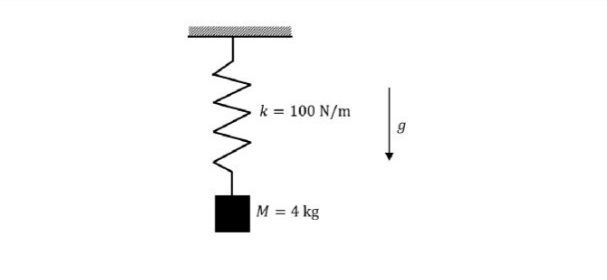
\includegraphics[width = \columnwidth]{figs/xe_71_f1.png}
\end{figure}
\hfill{(GATE 2023 XE)}\\
\solution
\begin{enumerate}
    \item Static deflection due to weight(sdw)\\
    let x be sdw.\\
    At mean position in equilibrium\\
     \ref{table:XE 71.t1}
    \begin{align}
        Mg&=kx\\
        x&=39.24cm
    \end{align}
     \item Time period of oscillation\\
        \begin{align}
           F&=-kx\\
           m\brak{\frac{d^2x}{dt^2}}&=-kx
     \end{align}
     Taking Laplace transform:
     \begin{align}
      X(s) &= \frac{ms x(0) + x'(0)}{ms^2 + k} \\
       X(s) &= \frac{1}{\sqrt{\frac{k}{m}}} \left( A \frac{s - i \sqrt{\frac{k}{m}}}{s^2 + \frac{k}{m}} + B \frac{s + i \sqrt{\frac{k}{m}}}{s^2 + \frac{k}{m}} \right) 
     \end{align}
     Taking Inverse Laplace Transform:\\
     \begin{align}
      x(t) &=A \left( B \sin(\sqrt{\frac{k}{m}}t) + C\cos(\sqrt{\frac{k}{m}}t) \right)\\
       x(t) &=P \left(\sin(\sqrt{\frac{k}{m}}t+Q) \right)\\
        x(t) &=P \sin(5t+Q) \\\label{XE_71_eq10}
       \end{align}
        Initial Conditions be at extreme  point of SHM
       \begin{align}
       x(0)&=0.3924=P sinQ\\\label{XE_71_eq11}  
       \frac{dx}{dt}&=0 \text{ at } t=0 \text{ (released from rest)} \\
       \frac{dx}{dt}&=5P\cos(Q)=0\label{XE_71_eq13}\\
       \end{align}   
solving \ref{XE_71_eq10} using \ref{XE_71_eq11} and \ref{XE_71_eq13}
       \begin{align}
      x(t)&=0.3924\sin\brak{5t+\frac{\pi}{2}}\text{ m}\\
      x(t)&=39.24 \sin\brak{5t+\frac{\pi}{2}} \text{ cm}
     \end{align}
    The static deflection due to weight and the time period of the oscillations,respectively are $39.24$ cm and $\frac{2\pi}{5}$ s
\end{enumerate}
 \begin{figure}[h!]
    \centering
    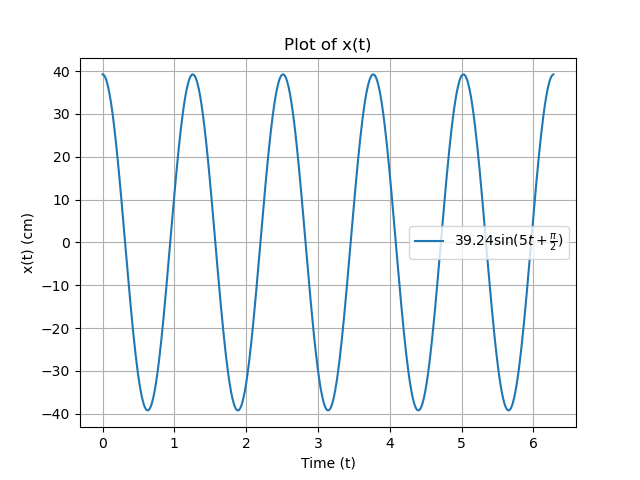
\includegraphics[width = \columnwidth]{figs/xe_71_f2.png}
\end{figure}
 \begin{table}[!ht]
    \centering
         \begin{tabular}{|c|c|} 
      \hline
\textbf{Variable}& \textbf{Value}\\\hline
         $R_1$ & $2\ohm$\\\hline
          $R_2$ &$1\ohm$\\\hline
          $L_1$  &$2$ H \\ \hline
         $L_2$  &$0.5$ H \\ \hline
    \end{tabular}

    \caption{input parameters}
     \label{XE 71.t1}
\end{table}
\end{document}

